%
% seilbahn.tex
%
% (c) 2024 Prof Dr Andreas Müller
%
\begin{figure}
\centering
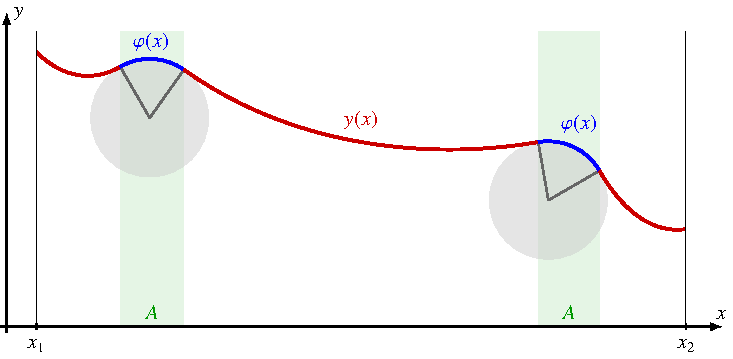
\includegraphics{chapters/050-nebenbedingungen/images/seilbahn.pdf}
\caption{Das Tragseil einer Seilbahn liegt in den Seilauflagerungen der
Zwischenstützen.
Da die Gesamtlänge des Seils vorgegeben ist, führt dies auf ein
Variationsproblem für die Funktion ${\color{darkred}y(x)}$ mit Nebenbedingungen.
In der Menge ${\color{darkgreen}A}$ liegt das Seil auf den Auflagerungen
auf und folgt dort der Nebenbedingung ${\color{blue}\varphi(x)}$.
\label{buch:nebenbedingungen:fig:seilbahn}}
\end{figure}
